\documentclass[twoside]{book}

% Packages required by doxygen
\usepackage{fixltx2e}
\usepackage{calc}
\usepackage{doxygen}
\usepackage[export]{adjustbox} % also loads graphicx
\usepackage{graphicx}
\usepackage[utf8]{inputenc}
\usepackage{makeidx}
\usepackage{multicol}
\usepackage{multirow}
\PassOptionsToPackage{warn}{textcomp}
\usepackage{textcomp}
\usepackage[nointegrals]{wasysym}
\usepackage[table]{xcolor}

% Font selection
\usepackage[T1]{fontenc}
\usepackage[scaled=.90]{helvet}
\usepackage{courier}
\usepackage{amssymb}
\usepackage{sectsty}
\renewcommand{\familydefault}{\sfdefault}
\allsectionsfont{%
  \fontseries{bc}\selectfont%
  \color{darkgray}%
}
\renewcommand{\DoxyLabelFont}{%
  \fontseries{bc}\selectfont%
  \color{darkgray}%
}
\newcommand{\+}{\discretionary{\mbox{\scriptsize$\hookleftarrow$}}{}{}}

% Page & text layout
\usepackage{geometry}
\geometry{%
  a4paper,%
  top=2.5cm,%
  bottom=2.5cm,%
  left=2.5cm,%
  right=2.5cm%
}
\tolerance=750
\hfuzz=15pt
\hbadness=750
\setlength{\emergencystretch}{15pt}
\setlength{\parindent}{0cm}
\setlength{\parskip}{3ex plus 2ex minus 2ex}
\makeatletter
\renewcommand{\paragraph}{%
  \@startsection{paragraph}{4}{0ex}{-1.0ex}{1.0ex}{%
    \normalfont\normalsize\bfseries\SS@parafont%
  }%
}
\renewcommand{\subparagraph}{%
  \@startsection{subparagraph}{5}{0ex}{-1.0ex}{1.0ex}{%
    \normalfont\normalsize\bfseries\SS@subparafont%
  }%
}
\makeatother

% Headers & footers
\usepackage{fancyhdr}
\pagestyle{fancyplain}
\fancyhead[LE]{\fancyplain{}{\bfseries\thepage}}
\fancyhead[CE]{\fancyplain{}{}}
\fancyhead[RE]{\fancyplain{}{\bfseries\leftmark}}
\fancyhead[LO]{\fancyplain{}{\bfseries\rightmark}}
\fancyhead[CO]{\fancyplain{}{}}
\fancyhead[RO]{\fancyplain{}{\bfseries\thepage}}
\fancyfoot[LE]{\fancyplain{}{}}
\fancyfoot[CE]{\fancyplain{}{}}
\fancyfoot[RE]{\fancyplain{}{\bfseries\scriptsize Generated by Doxygen }}
\fancyfoot[LO]{\fancyplain{}{\bfseries\scriptsize Generated by Doxygen }}
\fancyfoot[CO]{\fancyplain{}{}}
\fancyfoot[RO]{\fancyplain{}{}}
\renewcommand{\footrulewidth}{0.4pt}
\renewcommand{\chaptermark}[1]{%
  \markboth{#1}{}%
}
\renewcommand{\sectionmark}[1]{%
  \markright{\thesection\ #1}%
}

% Indices & bibliography
\usepackage{natbib}
\usepackage[titles]{tocloft}
\setcounter{tocdepth}{3}
\setcounter{secnumdepth}{5}
\makeindex

% Hyperlinks (required, but should be loaded last)
\usepackage{ifpdf}
\ifpdf
  \usepackage[pdftex,pagebackref=true]{hyperref}
\else
  \usepackage[ps2pdf,pagebackref=true]{hyperref}
\fi
\hypersetup{%
  colorlinks=true,%
  linkcolor=blue,%
  citecolor=blue,%
  unicode%
}

% Custom commands
\newcommand{\clearemptydoublepage}{%
  \newpage{\pagestyle{empty}\cleardoublepage}%
}

\usepackage{caption}
\captionsetup{labelsep=space,justification=centering,font={bf},singlelinecheck=off,skip=4pt,position=top}

%===== C O N T E N T S =====

\begin{document}

% Titlepage & ToC
\hypersetup{pageanchor=false,
             bookmarksnumbered=true,
             pdfencoding=unicode
            }
\pagenumbering{alph}
\begin{titlepage}
\vspace*{7cm}
\begin{center}%
{\Large Homework8 }\\
\vspace*{1cm}
{\large Generated by Doxygen 1.8.13}\\
\end{center}
\end{titlepage}
\clearemptydoublepage
\pagenumbering{roman}
\tableofcontents
\clearemptydoublepage
\pagenumbering{arabic}
\hypersetup{pageanchor=true}

%--- Begin generated contents ---
\chapter{Hierarchical Index}
\section{Class Hierarchy}
This inheritance list is sorted roughly, but not completely, alphabetically\+:\begin{DoxyCompactList}
\item $<$M\+K\+Annotation$>$\begin{DoxyCompactList}
\item \contentsline{section}{Res\+Annotation}{\pageref{interface_res_annotation}}{}
\end{DoxyCompactList}
\item N\+S\+Object\begin{DoxyCompactList}
\item \contentsline{section}{Res\+Annotation}{\pageref{interface_res_annotation}}{}
\end{DoxyCompactList}
\item $<$U\+I\+Application\+Delegate$>$\begin{DoxyCompactList}
\item \contentsline{section}{App\+Delegate}{\pageref{interface_app_delegate}}{}
\end{DoxyCompactList}
\item U\+I\+Responder\begin{DoxyCompactList}
\item \contentsline{section}{App\+Delegate}{\pageref{interface_app_delegate}}{}
\end{DoxyCompactList}
\item $<$U\+I\+Table\+View\+Data\+Source$>$\begin{DoxyCompactList}
\item \contentsline{section}{Restaurant\+View}{\pageref{interface_restaurant_view}}{}
\end{DoxyCompactList}
\item $<$U\+I\+Table\+View\+Delegate$>$\begin{DoxyCompactList}
\item \contentsline{section}{Restaurant\+View}{\pageref{interface_restaurant_view}}{}
\end{DoxyCompactList}
\item U\+I\+View\+Controller\begin{DoxyCompactList}
\item \contentsline{section}{Geographic\+View}{\pageref{interface_geographic_view}}{}
\item \contentsline{section}{Restaurant\+Map}{\pageref{interface_restaurant_map}}{}
\item \contentsline{section}{Restaurant\+View}{\pageref{interface_restaurant_view}}{}
\end{DoxyCompactList}
\end{DoxyCompactList}

\chapter{Class Index}
\section{Class List}
Here are the classes, structs, unions and interfaces with brief descriptions\+:\begin{DoxyCompactList}
\item\contentsline{section}{\hyperlink{interface_app_delegate}{App\+Delegate} }{\pageref{interface_app_delegate}}{}
\item\contentsline{section}{\hyperlink{interface_geographic_view}{Geographic\+View} }{\pageref{interface_geographic_view}}{}
\item\contentsline{section}{\hyperlink{interface_res_annotation}{Res\+Annotation} }{\pageref{interface_res_annotation}}{}
\item\contentsline{section}{\hyperlink{interface_restaurant_map}{Restaurant\+Map} }{\pageref{interface_restaurant_map}}{}
\item\contentsline{section}{\hyperlink{interface_restaurant_view}{Restaurant\+View} }{\pageref{interface_restaurant_view}}{}
\end{DoxyCompactList}

\chapter{Class Documentation}
\hypertarget{interface_app_delegate}{}\section{App\+Delegate Class Reference}
\label{interface_app_delegate}\index{App\+Delegate@{App\+Delegate}}
Inheritance diagram for App\+Delegate\+:\begin{figure}[H]
\begin{center}
\leavevmode
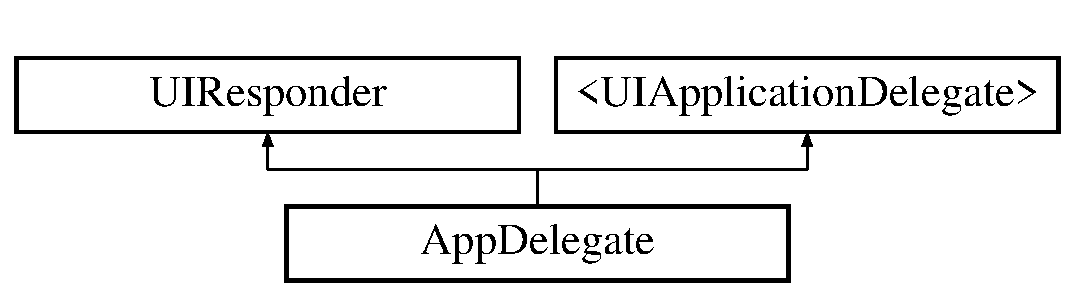
\includegraphics[height=2.000000cm]{interface_app_delegate}
\end{center}
\end{figure}
\subsection*{Properties}
\begin{DoxyCompactItemize}
\item 
\mbox{\Hypertarget{interface_app_delegate_acf48ac24125e688cac1a85445cd7fac2}\label{interface_app_delegate_acf48ac24125e688cac1a85445cd7fac2}} 
U\+I\+Window $\ast$ {\bfseries window}
\item 
\mbox{\Hypertarget{interface_app_delegate_a83fbaeeffead75ba8e2bc50360b34c18}\label{interface_app_delegate_a83fbaeeffead75ba8e2bc50360b34c18}} 
U\+I\+Tab\+Bar\+Controller $\ast$ {\bfseries tab}
\item 
\mbox{\Hypertarget{interface_app_delegate_a2d349e5d90658808241775ac95279afe}\label{interface_app_delegate_a2d349e5d90658808241775ac95279afe}} 
\hyperlink{interface_geographic_view}{Geographic\+View} $\ast$ {\bfseries vc1}
\item 
\mbox{\Hypertarget{interface_app_delegate_a8fc69d08569e5a6547ceeb5ba52d13e2}\label{interface_app_delegate_a8fc69d08569e5a6547ceeb5ba52d13e2}} 
\hyperlink{interface_restaurant_view}{Restaurant\+View} $\ast$ {\bfseries vc2}
\item 
\mbox{\Hypertarget{interface_app_delegate_a33d5e0a6fbd7ae8a3142f03622551b3a}\label{interface_app_delegate_a33d5e0a6fbd7ae8a3142f03622551b3a}} 
U\+I\+Navigation\+Controller $\ast$ {\bfseries nav2}
\end{DoxyCompactItemize}


The documentation for this class was generated from the following file\+:\begin{DoxyCompactItemize}
\item 
Homework8/App\+Delegate.\+h\end{DoxyCompactItemize}

\hypertarget{interface_geographic_view}{}\section{Geographic\+View Class Reference}
\label{interface_geographic_view}\index{Geographic\+View@{Geographic\+View}}
Inheritance diagram for Geographic\+View\+:\begin{figure}[H]
\begin{center}
\leavevmode
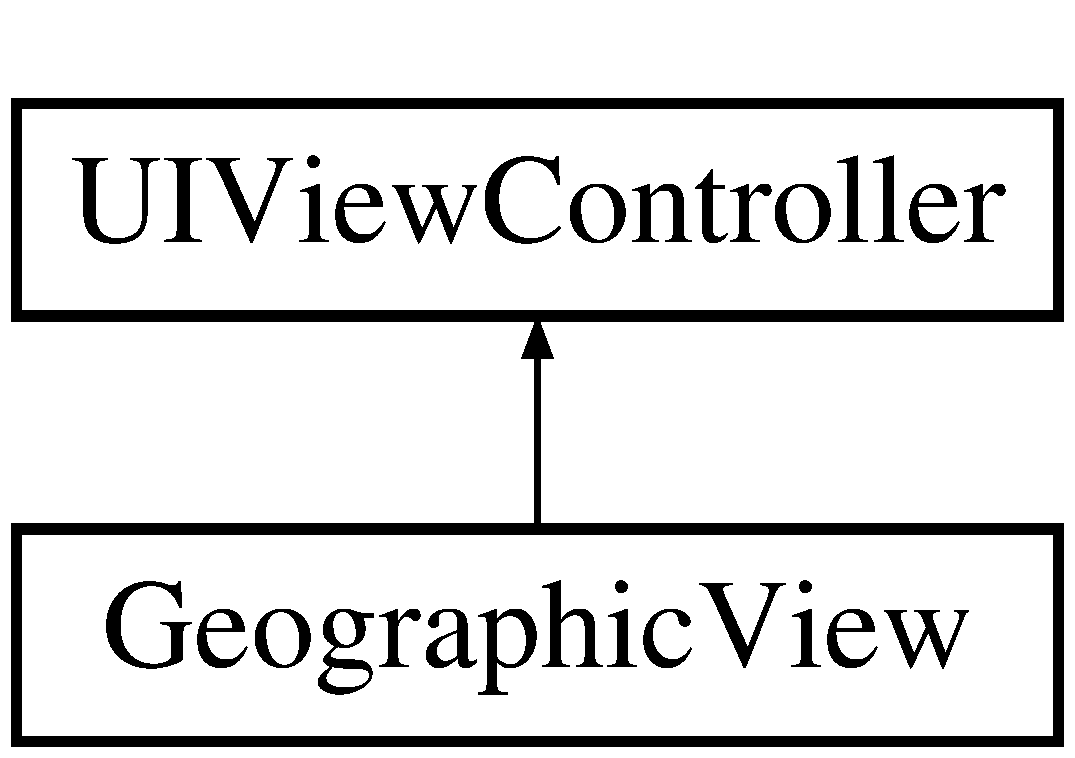
\includegraphics[height=2.000000cm]{interface_geographic_view}
\end{center}
\end{figure}
\subsection*{Protected Attributes}
\begin{DoxyCompactItemize}
\item 
\mbox{\Hypertarget{interface_geographic_view_ac59ae9d08065e3932794fd3465dd5711}\label{interface_geographic_view_ac59ae9d08065e3932794fd3465dd5711}} 
C\+L\+Location\+Manager $\ast$ {\bfseries manager}
\item 
\mbox{\Hypertarget{interface_geographic_view_a1d15140f77e7b613af0dbc818777b5b7}\label{interface_geographic_view_a1d15140f77e7b613af0dbc818777b5b7}} 
U\+I\+Image\+View $\ast$ {\bfseries vcompass}
\item 
\mbox{\Hypertarget{interface_geographic_view_ac4c2ade1c371a5b77d532317331ce072}\label{interface_geographic_view_ac4c2ade1c371a5b77d532317331ce072}} 
U\+I\+Text\+View $\ast$ {\bfseries vlat}
\item 
\mbox{\Hypertarget{interface_geographic_view_a09fbfe2e1d8b1826626c73725e01a238}\label{interface_geographic_view_a09fbfe2e1d8b1826626c73725e01a238}} 
U\+I\+Text\+View $\ast$ {\bfseries vlon}
\item 
\mbox{\Hypertarget{interface_geographic_view_a6c91f0a9699be7ba59bf7690027e20e9}\label{interface_geographic_view_a6c91f0a9699be7ba59bf7690027e20e9}} 
U\+I\+Text\+View $\ast$ {\bfseries vdir}
\item 
\mbox{\Hypertarget{interface_geographic_view_ac0e4fd8402f5ca0aac7f7a8d55cbb635}\label{interface_geographic_view_ac0e4fd8402f5ca0aac7f7a8d55cbb635}} 
U\+I\+Text\+View $\ast$ {\bfseries valt}
\item 
\mbox{\Hypertarget{interface_geographic_view_af88e600b7637adc61d79f24dfa4e9d00}\label{interface_geographic_view_af88e600b7637adc61d79f24dfa4e9d00}} 
U\+I\+Text\+View $\ast$ {\bfseries vspeed}
\end{DoxyCompactItemize}


The documentation for this class was generated from the following file\+:\begin{DoxyCompactItemize}
\item 
Homework8/Geographic\+View.\+h\end{DoxyCompactItemize}

\hypertarget{interface_res_annotation}{}\section{Res\+Annotation Class Reference}
\label{interface_res_annotation}\index{Res\+Annotation@{Res\+Annotation}}
Inheritance diagram for Res\+Annotation\+:\begin{figure}[H]
\begin{center}
\leavevmode
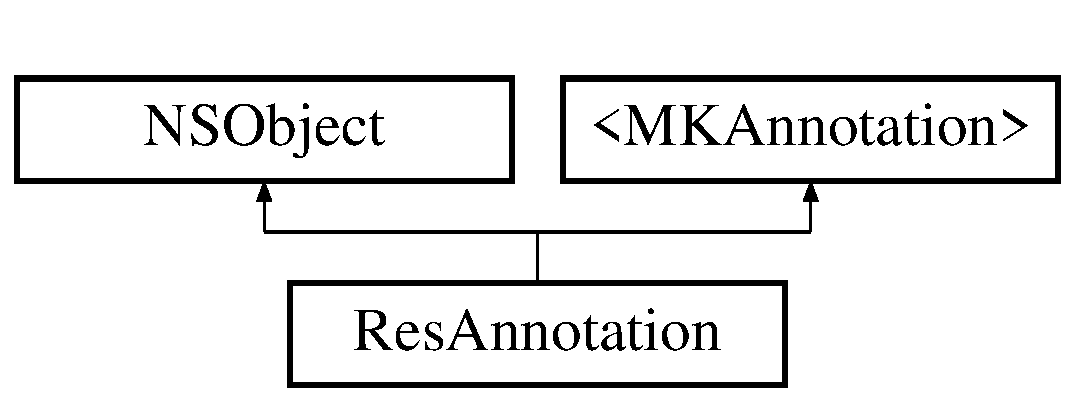
\includegraphics[height=2.000000cm]{interface_res_annotation}
\end{center}
\end{figure}
\subsection*{Properties}
\begin{DoxyCompactItemize}
\item 
\mbox{\Hypertarget{interface_res_annotation_af3510c3c75b05b25e15d94a5a07b289f}\label{interface_res_annotation_af3510c3c75b05b25e15d94a5a07b289f}} 
C\+L\+Location\+Coordinate2D {\bfseries coordinate}
\item 
\mbox{\Hypertarget{interface_res_annotation_aa8e6337d913abfebf2e67b5569fd9c89}\label{interface_res_annotation_aa8e6337d913abfebf2e67b5569fd9c89}} 
N\+S\+String $\ast$ {\bfseries title}
\item 
\mbox{\Hypertarget{interface_res_annotation_a51cff184d1d0f94f4f51e889acd4a25b}\label{interface_res_annotation_a51cff184d1d0f94f4f51e889acd4a25b}} 
N\+S\+String $\ast$ {\bfseries subtitle}
\end{DoxyCompactItemize}


The documentation for this class was generated from the following file\+:\begin{DoxyCompactItemize}
\item 
Homework8/Res\+Annotation.\+h\end{DoxyCompactItemize}

\hypertarget{interface_restaurant_map}{}\section{Restaurant\+Map Class Reference}
\label{interface_restaurant_map}\index{Restaurant\+Map@{Restaurant\+Map}}
Inheritance diagram for Restaurant\+Map\+:\begin{figure}[H]
\begin{center}
\leavevmode
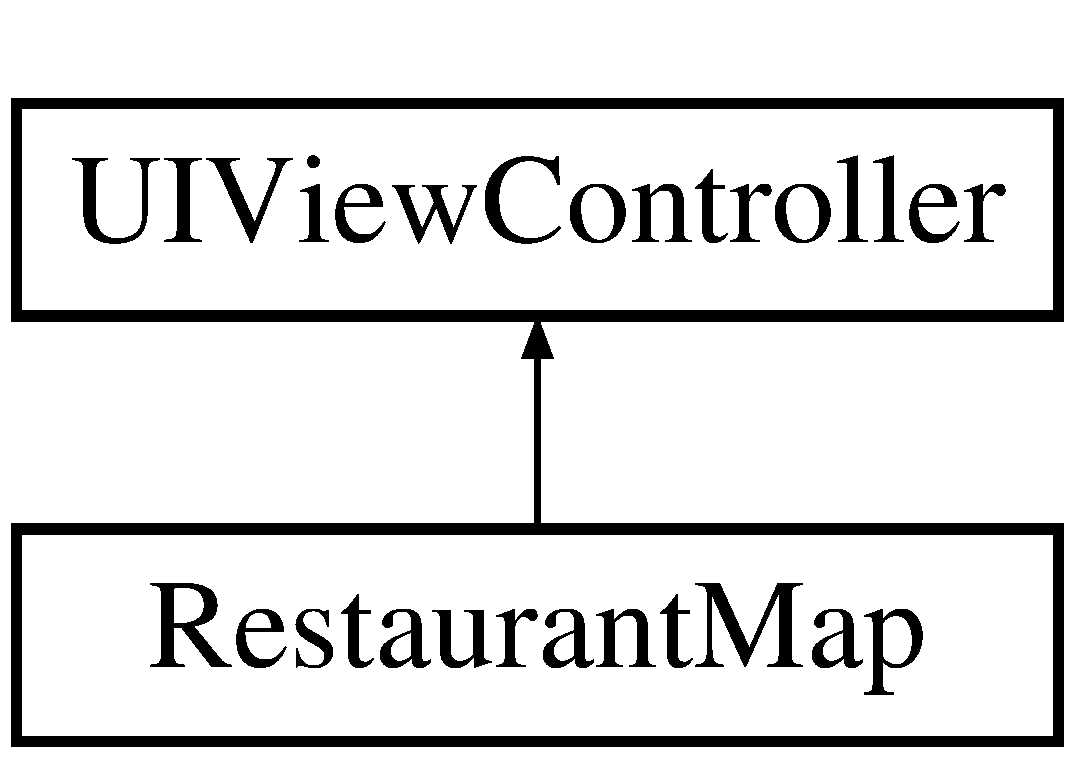
\includegraphics[height=2.000000cm]{interface_restaurant_map}
\end{center}
\end{figure}
\subsection*{Instance Methods}
\begin{DoxyCompactItemize}
\item 
\mbox{\Hypertarget{interface_restaurant_map_a1fd46f905bd580138d4436f79db70963}\label{interface_restaurant_map_a1fd46f905bd580138d4436f79db70963}} 
(void) -\/ {\bfseries init\+Controls}
\end{DoxyCompactItemize}
\subsection*{Protected Attributes}
\begin{DoxyCompactItemize}
\item 
\mbox{\Hypertarget{interface_restaurant_map_ad251a89fa2a9b310ea303a6a6fd9e5e2}\label{interface_restaurant_map_ad251a89fa2a9b310ea303a6a6fd9e5e2}} 
U\+I\+Text\+View $\ast$ {\bfseries vname}
\item 
\mbox{\Hypertarget{interface_restaurant_map_adcd0272bcffdad62b4cf509f4d06b757}\label{interface_restaurant_map_adcd0272bcffdad62b4cf509f4d06b757}} 
U\+I\+Image\+View $\ast$ {\bfseries vimage}
\item 
\mbox{\Hypertarget{interface_restaurant_map_a7eaa0497cd3c4f523030df6fcfde01d9}\label{interface_restaurant_map_a7eaa0497cd3c4f523030df6fcfde01d9}} 
U\+I\+Text\+View $\ast$ {\bfseries vlink}
\item 
\mbox{\Hypertarget{interface_restaurant_map_a5dac46b85d34c5c1ad755e5f89fc3ef1}\label{interface_restaurant_map_a5dac46b85d34c5c1ad755e5f89fc3ef1}} 
U\+I\+Text\+View $\ast$ {\bfseries vinfo}
\item 
\mbox{\Hypertarget{interface_restaurant_map_af3daff8212c5ec90de89b4a6a2b4f636}\label{interface_restaurant_map_af3daff8212c5ec90de89b4a6a2b4f636}} 
M\+K\+Map\+View $\ast$ {\bfseries vmap}
\item 
\mbox{\Hypertarget{interface_restaurant_map_a23340b6483580b754a7a5a639c58c161}\label{interface_restaurant_map_a23340b6483580b754a7a5a639c58c161}} 
C\+L\+Location\+Manager $\ast$ {\bfseries manager}
\item 
\mbox{\Hypertarget{interface_restaurant_map_aae6e6967309f8eed8bae0a7e63d2e6ae}\label{interface_restaurant_map_aae6e6967309f8eed8bae0a7e63d2e6ae}} 
C\+L\+Geocoder $\ast$ {\bfseries geocoder}
\end{DoxyCompactItemize}
\subsection*{Properties}
\begin{DoxyCompactItemize}
\item 
\mbox{\Hypertarget{interface_restaurant_map_ae4fafff89e6b2244aac270b7c7551b77}\label{interface_restaurant_map_ae4fafff89e6b2244aac270b7c7551b77}} 
N\+S\+String $\ast$ {\bfseries sname}
\item 
\mbox{\Hypertarget{interface_restaurant_map_a600869b5a5556d9e4f3d734271dc09ed}\label{interface_restaurant_map_a600869b5a5556d9e4f3d734271dc09ed}} 
double {\bfseries dlat}
\item 
\mbox{\Hypertarget{interface_restaurant_map_acf5fcb7055f9266af08d0586464916ca}\label{interface_restaurant_map_acf5fcb7055f9266af08d0586464916ca}} 
double {\bfseries dlon}
\item 
\mbox{\Hypertarget{interface_restaurant_map_a7e18d9bd9127d6d190b19e458b65f579}\label{interface_restaurant_map_a7e18d9bd9127d6d190b19e458b65f579}} 
N\+S\+String $\ast$ {\bfseries simage}
\item 
\mbox{\Hypertarget{interface_restaurant_map_ab4730030e43bb99f5c54492e55d73630}\label{interface_restaurant_map_ab4730030e43bb99f5c54492e55d73630}} 
N\+S\+String $\ast$ {\bfseries slink}
\item 
\mbox{\Hypertarget{interface_restaurant_map_a5540509713cccf07a4a4a865fd044cfd}\label{interface_restaurant_map_a5540509713cccf07a4a4a865fd044cfd}} 
N\+S\+String $\ast$ {\bfseries sinfo}
\end{DoxyCompactItemize}


The documentation for this class was generated from the following files\+:\begin{DoxyCompactItemize}
\item 
Homework8/Restaurant\+Map.\+h\item 
Homework8/Restaurant\+Map.\+m\end{DoxyCompactItemize}

\hypertarget{interface_restaurant_view}{}\section{Restaurant\+View Class Reference}
\label{interface_restaurant_view}\index{Restaurant\+View@{Restaurant\+View}}
Inheritance diagram for Restaurant\+View\+:\begin{figure}[H]
\begin{center}
\leavevmode
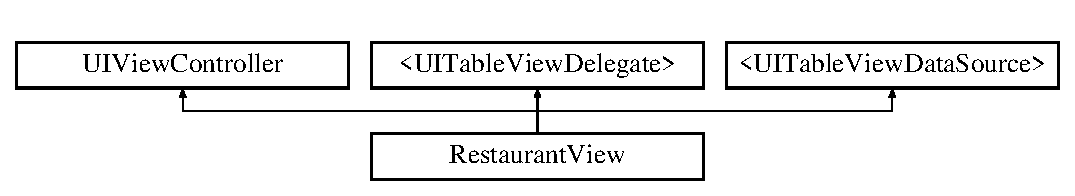
\includegraphics[height=2.000000cm]{interface_restaurant_view}
\end{center}
\end{figure}
\subsection*{Protected Attributes}
\begin{DoxyCompactItemize}
\item 
\mbox{\Hypertarget{interface_restaurant_view_a651ab7f6723ad88045d6a83026c3f8f2}\label{interface_restaurant_view_a651ab7f6723ad88045d6a83026c3f8f2}} 
N\+S\+Mutable\+Array $\ast$ {\bfseries restaurants}
\item 
\mbox{\Hypertarget{interface_restaurant_view_afab1648b171ef7a86be28bbaca91f0f8}\label{interface_restaurant_view_afab1648b171ef7a86be28bbaca91f0f8}} 
U\+I\+Table\+View $\ast$ {\bfseries table}
\end{DoxyCompactItemize}


The documentation for this class was generated from the following file\+:\begin{DoxyCompactItemize}
\item 
Homework8/Restaurant\+View.\+h\end{DoxyCompactItemize}

%--- End generated contents ---

% Index
\backmatter
\newpage
\phantomsection
\clearemptydoublepage
\addcontentsline{toc}{chapter}{Index}
\printindex

\end{document}
